\documentclass[11pt]{article}
\usepackage[margin=1in]{geometry}
\usepackage[T1]{fontenc}
\usepackage{lmodern}
\usepackage{amsmath,amssymb}
\usepackage{booktabs}
\usepackage{siunitx}
\usepackage{graphicx}
\usepackage{xcolor}
\usepackage[numbers,sort&compress]{natbib}
\usepackage{url}
\usepackage[colorlinks=true,linkcolor=blue!50!black,citecolor=blue!50!black,urlcolor=blue!50!black]{hyperref}
\usepackage{cleveref}

% GENERATED by figures/make_figures.py from results/*.json -- do not edit
\newcommand{\provisional}{1}
\newcommand{\benchSource}{quick.json}
\newcommand{\gpuName}{NVIDIA GeForce RTX 3070 Laptop GPU}
\newcommand{\copyBW}{361}
\newcommand{\fmaPeak}{12.9}
\newcommand{\bestRate}{308}
\newcommand{\bestBackend}{cupy-cuda-c}
\newcommand{\bestVariant}{full}
\newcommand{\bestN}{32{,}000}
\newcommand{\bestPctCopy}{30}
\newcommand{\bestPctSpec}{24}
\newcommand{\bestPctFlops}{5}
\newcommand{\bestTauDay}{4{,}164{,}280}
\newcommand{\bestNsDay}{8{,}980}
\newcommand{\bestBytes}{348}
\newcommand{\bestListLen}{75.0}
\newcommand{\refN}{32{,}000}
\newcommand{\refTorchEager}{3.7}
\newcommand{\refTorchEagerPct}{0}
\newcommand{\refTorchCompile}{26.8}
\newcommand{\refTorchCompilePct}{3}
\newcommand{\refTriton}{218.6}
\newcommand{\refTritonPct}{21}
\newcommand{\refWarp}{266.3}
\newcommand{\refWarpPct}{26}
\newcommand{\refNumba}{255.8}
\newcommand{\refNumbaPct}{25}
\newcommand{\refCupy}{308.5}
\newcommand{\refCupyPct}{30}
\newcommand{\ratioTriton}{67}
\newcommand{\ratioWarp}{86}
\newcommand{\ratioNumba}{59}
\newcommand{\numpySmall}{0.16}
\newcommand{\ablHalf}{157}
\newcommand{\ablHalfRatio}{0.51}
\newcommand{\ablFused}{304}
\newcommand{\ablFusedRatio}{0.99}
\newcommand{\forceErrMax}{5.5e-06}
\newcommand{\forceErrMin}{5.4e-06}
\newcommand{\forceErrMixed}{9.1e-07}
\newcommand{\forceErrFpSixtyFour}{8e-16}
\newcommand{\forceN}{4{,}000}
\newcommand{\inljZeroTemp}{1.4400000}
\newcommand{\inljHundredTemp}{0.7586}
\newcommand{\inljHundredTempStd}{0.0030}
\newcommand{\inljZeroEpot}{-6.7733674}
\newcommand{\inljHundredEpot}{-5.7602}
\newcommand{\inljHundredEpotStd}{0.0044}
\newcommand{\inljZeroEtot}{-4.6134349}
\newcommand{\inljHundredEtot}{-4.6224}
\newcommand{\inljHundredEtotStd}{0.0001}
\newcommand{\inljZeroPress}{-5.0197081}
\newcommand{\inljHundredPress}{0.1942}
\newcommand{\inljHundredPressStd}{0.0174}
\newcommand{\inljSeeds}{8}
\newcommand{\inljNeigh}{37.554}
\newcommand{\inljBuilds}{5}


\newcommand{\pymd}{\texttt{pymd}}
\newcommand{\yamd}{\texttt{yamd}}
\sisetup{group-separator={,},group-minimum-digits=4}

\title{Lennard-Jones molecular dynamics at GPU speed from pure Python:\\
an optimization ladder from NumPy to Triton, Warp, Numba and CUDA C}
\author{Walid Hemati\\ \small Independent researcher}
\date{October 2026}

\begin{document}
\maketitle

\ifnum\provisional=1
\begin{center}
\fcolorbox{red}{red!8}{\parbox{0.92\linewidth}{\centering\bfseries\color{red!70!black}
PROVISIONAL NUMBERS --- performance figures come from a development run on a shared GPU
(\texttt{results/\benchSource}) and will be replaced by the final serial benchmark.}}
\end{center}
\fi

\begin{abstract}
We ask whether a molecular-dynamics (MD) code written entirely in Python can use a GPU as
efficiently as hand-written CUDA. \pymd{} is a Lennard-Jones (LJ) and second-moment
(Gupta/EAM) MD engine whose time-stepping logic is written once and whose hot loops exist as
interchangeable backends: NumPy, PyTorch (eager and \texttt{torch.compile}), Triton, NVIDIA
Warp, Numba-CUDA and hand-written CUDA C compiled at run time through CuPy/NVRTC. All
backends share GPU cell lists built by counting sort, Verlet neighbor lists with a skin, and
spatial atom sorting. On the LAMMPS \texttt{in.lj} melt benchmark, scaled up to four million
atoms on a laptop RTX~3070, the fastest variant (\bestBackend/\bestVariant) reaches
\bestRate{}~million atom-steps per second at $N=\bestN$, i.e.\ \bestPctCopy\% of the measured
copy bandwidth under a minimal-traffic model. The Python kernel languages run the same
algorithm at \ratioTriton\% (Triton), \ratioWarp\% (Warp) and \ratioNumba\% (Numba) of the
throughput of the CUDA C reference at $N=\refN$. Correctness is established against a float64
NumPy oracle (relative force error $\le\forceErrMax$ in single precision), the
LAMMPS reference log of \texttt{in.lj}, NIST reference simulation data, the
Johnson--Zollweg--Gubbins equation of state, and the author's earlier C++ code \yamd{},
whose forces \pymd{} reproduces to $\yamdForceDiff$. We also build LAMMPS (GPU and KOKKOS
packages) and HOOMD-blue and run them on the same GPU on the same, cross-verified system.
\end{abstract}

\section{Introduction}
Classical MD of simple liquids is the canonical short-range particle workload: each step
gathers the positions of ${\sim}50$--$100$ neighbors per atom, evaluates a cheap pair
function, and accumulates forces. Production GPU codes such as LAMMPS' GPU and KOKKOS
packages~\cite{brown2011lammpsgpu,thompson2022lammps} and HOOMD-blue~\cite{anderson2008hoomd,
glaser2015,anderson2020hoomd} implement this in CUDA C++. In parallel, a family of Python GPU
programming tools has matured: Triton~\cite{tillet2019triton}, NVIDIA
Warp~\cite{warp2022}, Numba~\cite{lam2015numba}, CuPy~\cite{okuta2017cupy} and
PyTorch~\cite{paszke2019pytorch} with its compiler \texttt{torch.compile}~\cite{ansel2024pytorch2}.
This paper measures how close each of them comes to the hardware limit on the same problem,
with the same algorithms, on the same GPU.

\pymd{} is the Python successor of \yamd{}~\cite{yamd}, the author's C++/Eigen MD code
(LJ direct summation, velocity Verlet, Berendsen thermostat, cell-based neighbor lists, and a
Gupta potential for gold clusters). \pymd{} mirrors \yamd's features and test cases and adds
periodic boundaries, GPU neighbor search and a Langevin thermostat. Contributions:
\begin{itemize}
\item An MD engine with one integrator and a registry of 23 backend/variant combinations
  spanning seven programming models, all validated against one float64 oracle
  (\cref{sec:impl,sec:validation}).
\item A minimal memory-traffic and flop model per atom-step for Verlet-list MD, used to report
  every throughput as a fraction of the measured copy bandwidth and FMA peak
  (\cref{sec:traffic}).
\item An optimization ladder with ablations of spatial sorting (none, cell order, Morton
  order), full versus half (atomic) neighbor lists, kernel fusion, and precision (fp32, mixed,
  fp64) (\cref{sec:perf}).
\item Validation against the LAMMPS \texttt{in.lj} reference output, NIST SRSW Monte Carlo
  data~\cite{nist_srsw}, the JZG equation of state~\cite{johnson1993lj}, and a same-machine
  cross-check and head-to-head with the C++ code \yamd{} (\cref{sec:validation,sec:yamd}).
\item A same-GPU head-to-head with LAMMPS (GPU and KOKKOS packages, double and single
  precision) and HOOMD-blue (conda-forge double-precision build and a single-precision source
  build), after checking that all codes integrate an identical initial state to the same
  trajectory (\cref{sec:counterparts}).
\end{itemize}

\section{Background and related work}
GPU MD with Verlet lists was established by Anderson et al.~\cite{anderson2008hoomd}, who
already used space-filling-curve (Hilbert) reordering of particles for memory locality, and
for LAMMPS by Brown et al.~\cite{brown2011lammpsgpu}; Glaser et al.\ studied strong scaling
of HOOMD-blue across GPUs~\cite{glaser2015}. Python front ends are common (HOOMD-blue v2+~\cite{anderson2020hoomd},
OpenMM~\cite{eastman2024openmm}), but their kernels are C++/CUDA. JAX MD~\cite{schoenholz2020jaxmd}
expresses MD in a differentiable array language. Our question is different: what fraction of
the GPU's capability do the Python \emph{kernel} languages themselves reach? We answer with the
roofline method~\cite{williams2009roofline}. Textbook background on the algorithms we use is
in Allen \& Tildesley~\cite{allen2017} and Frenkel \& Smit~\cite{frenkel2002}.

\section{Method}\label{sec:method}
\paragraph{Model.} Atoms interact through the LJ potential
$u(r)=4\epsilon[(\sigma/r)^{12}-(\sigma/r)^6]$ truncated at $r_c$ (optionally shifted so that
$u(r_c)=0$), in reduced units $\sigma=\epsilon=m=k_B=1$, with periodic boundaries and the
minimum-image convention. For comparisons with full-LJ data we add the standard long-range
corrections~\cite{allen2017}. Metals use the second-moment tight-binding (Gupta) potential
$E_i=\sum_j A e^{-p(r_{ij}/r_0-1)}-\big(\sum_j\xi^2e^{-2q(r_{ij}/r_0-1)}\big)^{1/2}$
\cite{ducastelle1970,gupta1981,cleri1993} with \yamd's gold parameters ($A=0.2061$\,eV,
$\xi=1.790$\,eV, $p=10.229$, $q=4.036$, $r_0=4.079/\sqrt2$\,\AA, cutoff 10\,\AA), evaluated in two
passes (density, then force).

\paragraph{Integration.} Velocity Verlet~\cite{swope1982} with the two half kicks of
consecutive steps fused into one kick-drift kernel; the fused variants use the equivalent
leapfrog form so that force, kick and drift happen in a single kernel per step (positions are
double-buffered). Thermostats: Berendsen velocity rescaling~\cite{berendsen1984} (as in
\yamd) and Langevin dynamics with the BAOAB splitting~\cite{leimkuhler2013}.

\paragraph{Neighbor search.} At each rebuild, positions are wrapped into the box and binned
into cells of edge $\ge r_c+r_s$ ($r_s$: skin). A counting sort (atomic histogram, exclusive
scan, atomic-slot scatter) yields cell start offsets; by default the atom arrays are then
physically permuted into cell order, so that neighbors in space are neighbors in memory. The
cell key is either row-major or a Morton (Z-order) interleave of the cell coordinates. A
Verlet list of all $j$ with $|r_{ij}|<r_c+r_s$ is then built over the 27-cell stencil with one
thread per atom and stored neighbor-major ($\texttt{nl}[k N+i]$) for coalesced reads; an
overflow flag triggers a resize and rebuild. The list is rebuilt every $n_{\mathrm{every}}$
steps, unconditionally (LAMMPS ``\texttt{check no}'') or only if some atom moved more than
$r_s/2$ (``\texttt{check yes}'').

\paragraph{Benchmark problem.} We use the LAMMPS \texttt{bench/in.lj} melt~\cite{lammps_inlj}:
FCC lattice at $\rho^*=0.8442$, initial $T^*=1.44$, $r_c=2.5\sigma$, $r_s=0.3\sigma$, list rebuilt
every 20 steps without a check, NVE, $\Delta t=0.005\tau$. The original has 32{,}000 atoms;
we scale it from 4{,}000 to 4{,}000{,}000. Atom order is randomly shuffled at $t=0$ so that
sorting has to earn its benefit. The metric is atom-steps per second (LAMMPS'
``atom-step/s''); we also give $\tau$/day and, with the argon mapping
$\sigma=0.3405$\,nm, $\epsilon/k_B=119.8$\,K, $m=39.948$\,u ($\tau\approx2.156$\,ps), ns/day.

\section{Implementation: the optimization ladder}\label{sec:impl}
A backend implements nine primitives (rebuild, forces with or without energy/virial,
kick-drift, max displacement, kinetic energy, velocity scaling, OU noise, up/download); the
driver in \texttt{engine.py} implements Verlet, the rebuild schedule and the thermostats once.
\begin{description}
\item[NumPy] (float64, CPU): cell list via \texttt{argsort}, padded cell table, vectorized
  candidate generation per stencil offset, half pair list, \texttt{np.bincount} scatter. This is
  also the correctness oracle (together with an $O(N^2)$ direct sum).
\item[PyTorch eager] a padded atom-major $(N,M)$ neighbor matrix and a \emph{gather}
  formulation, \texttt{x[nl]}, processed in chunks to bound the $(N,M)$ intermediates.
\item[\texttt{torch.compile}] the same code compiled by TorchInductor. Writing the gather per
  Cartesian component (structure of arrays) let Inductor fuse gather, pair math and reduction
  into one generated Triton kernel; the array-of-structures version was ${\sim}3\times$ slower.
\item[Triton] hand-written kernels: block of 128 atoms per program, a dynamic loop to the
  block's maximum neighbor count, constexpr switches for energy, fusion and half lists.
  Rebuild-time glue (key sort, permutation) uses PyTorch.
\item[Warp] a hand-written counting-sort cell list, list build and force kernels, and two
  variants using Warp's built-in \texttt{HashGrid}: \texttt{hashgrid} (no Verlet list; grid
  rebuilt and queried every step) and \texttt{hashgrid-verlet} (grid used only to build the
  list). With a cubic box and $\lfloor L/r\rfloor$ cells per side, the hash wrap coincides with
  the periodic wrap.
\item[Numba-CUDA] the same kernel set in \texttt{@cuda.jit}, including a single-block scan.
\item[CuPy CUDA C] the hand-written reference, compiled by NVRTC, with \texttt{float4}
  positions and templated precision. Variants: \texttt{full}, \texttt{full-fused},
  \texttt{half-atomic} (Newton's third law with \texttt{atomicAdd}), \texttt{full-tpa2/4}
  (two or four threads per atom, warp-shuffle reduction), \texttt{full-morton},
  \texttt{full-nosort}, \texttt{full-mixed} (fp64 positions, velocities and integration; fp32 pair math and per-atom sums),
  \texttt{full-fp64}, and a shared-memory tiled $O(N^2)$ \texttt{allpairs}.
\end{description}

\subsection{Traffic and flop model}\label{sec:traffic}
For one Verlet-list step the compulsory DRAM traffic per atom is: read $\mathbf{x}_i$, read
and write $\mathbf{v}_i$, write $\mathbf{x}_i$ (12 words) and read the stored list, 4 bytes per
entry: $B=48+4\,n_\ell$ bytes in fp32 ($96+4n_\ell$ with fp64 storage), where $n_\ell$ is the
measured mean list length (${\approx}75$ for a full list at $r_c+r_s=2.8\sigma$, half that for a
half list). Neighbor positions are assumed to come from cache and the amortized rebuild
traffic is ignored, so the effective bandwidth $R\cdot B$ is a lower bound and never
inflated. Each list entry costs 20 flop (difference, minimum image, $r^2$; FMA = 2 flop) and
each pair inside $r_c$ (a fraction $(r_c/(r_c+r_s))^3$ of entries) 13 more. The arithmetic
intensity is ${\approx}6$ flop/byte, well left of the ridge point
($\fmaPeak$\,TFLOP/s $/$ \copyBW\,GB/s), so the bandwidth roofline is the relevant ceiling.
Ceilings: \copyBW\,GB/s device-to-device copy (\texttt{torch} \texttt{copy\_}, read+write),
448\,GB/s specification, and \fmaPeak\,TFLOP/s from our fp32 FMA microbenchmark.

\section{Validation}\label{sec:validation}
\paragraph{Forces.} For a liquid configuration ($N=\forceN$, $\rho^*=0.8442$, $T^*=0.722$) every
variant is compared with the float64 NumPy direct sum (\cref{fig:validation}a). All
single-precision variants agree to $\max_i|\Delta F_i|/\max_i|F_i|$ between \forceErrMin{} and
\forceErrMax; mixed precision reaches \forceErrMixed{} and fp64 \forceErrFpSixtyFour.
The CPU tests port \yamd's GoogleTest cases (finite-difference LJ and Gupta forces, constant-force
Verlet, Berendsen relaxation, neighbor-list cases) and run in CI.

\paragraph{LAMMPS \texttt{in.lj}.} Step 0 is deterministic: on the GPU we obtain
$E_\mathrm{pair}=\inljZeroEpot$ and $P=\inljZeroPress$ versus LAMMPS'
$-6.7733681$ and $-5.0197073$ (the float64 NumPy path matches all digits). After 100 steps the
trajectories depend on the random velocities, so we average \inljSeeds{} seeds drawn, like
LAMMPS' default, from a uniform distribution: $T=\inljHundredTemp\pm\inljHundredTempStd$,
$E_\mathrm{pair}=\inljHundredEpot\pm\inljHundredEpotStd$,
$E_\mathrm{tot}=\inljHundredEtot\pm\inljHundredEtotStd$, $P=\inljHundredPress\pm\inljHundredPressStd$
(mean $\pm$ seed-to-seed standard deviation), against LAMMPS' single trajectory $0.7574531$,
$-5.7585055$, $-4.6223613$, $0.20726105$. The half-list length is \inljNeigh{} (LAMMPS:
37.588531) with \inljBuilds{} rebuilds (LAMMPS: 5). (With Gaussian velocities the step-100
pressure is systematically higher, a reminder that the 100-step melt is not equilibrated.)

\paragraph{Energy conservation.} NVE runs of a $N=4000$ liquid ($\rho^*=0.8442$, $T^*\approx0.72$,
shifted potential, list checked every step) show the expected $\Delta t^2$ scaling of the
energy fluctuation for $\Delta t\ge0.003$ (fitted exponent \fluctSlope,
\cref{fig:validation}b); at smaller steps the fluctuation levels off, as expected for a
potential whose force is discontinuous at $r_c$. Over $\driftTime\,\tau$ at $\Delta t=0.005$
the fitted linear drifts are \driftSingle{} (fp32), \driftMixed{} (mixed) and \driftDouble{}
(fp64) $\epsilon/\tau$ per atom (\cref{fig:validation}c). These are all small compared with the
fluctuation and of similar size for the three precisions; repeated runs show energy wander of
${\sim}10^{-4}\epsilon$ per atom over $200\tau$ for every precision, so on this time scale the
error budget is set by time discretization and the force cutoff, not by single-precision
round-off.

\paragraph{Structure.} \Cref{fig:rdf} shows $g(r)$ of the dense liquid $\rho^*=0.8442$,
$T^*=0.722$ ($r_c=3\sigma$, Langevin NVT). The first peak is at $r=\rdfPeakR\sigma$ with
height \rdfPeakG. We did not find tabulated literature $g(r)$ values for this state that we
could verify (Verlet's 1968 tables~\cite{verlet1968} were not accessible to us), so we test
$g(r)$ through thermodynamic consistency instead: the energy route
$U/N=2\pi\rho\int u\,g\,r^2\mathrm dr=\rdfUroute$ equals the direct average
$\rdfUdirect\pm\rdfUdirectErr$, the virial route gives $P=\rdfProute$ versus
$\rdfPdirect\pm\rdfPdirectErr$, and the energy route with the full potential,
\rdfUrouteFull, agrees with the JZG equation of state~\cite{johnson1993lj}, \rdfUjzg.

\paragraph{Equation of state.} At the \eosNpts{} liquid NIST SRSW Monte Carlo state points
($T^*=0.85,0.90$, $\rho^*=0.776$--$0.90$, $N=500$, $r_c=3\sigma$ + long-range
corrections~\cite{nist_srsw}) our Langevin NVT averages agree with NIST to within
\eosMaxRelU\% in energy and \eosMaxAbsP{} in pressure (largest deviation \eosMaxZP{} combined
standard errors), and both agree with JZG (\cref{fig:validation}d). We transcribed the 32 JZG
coefficients from NIST's \texttt{teqp}; they reproduce the NIST data, which is an independent
check of the transcription.

\paragraph{EAM gold.} For a perturbed Mackay icosahedron~\cite{mackay1962} of \eamN{} Au
atoms the GPU fp32 Gupta forces match float64 to \eamForceErr, and NVE with $\Delta t=1$\,fs
conserves energy to \eamDrift\,eV/atom over 2\,ps.

\begin{figure}[htbp]
\centering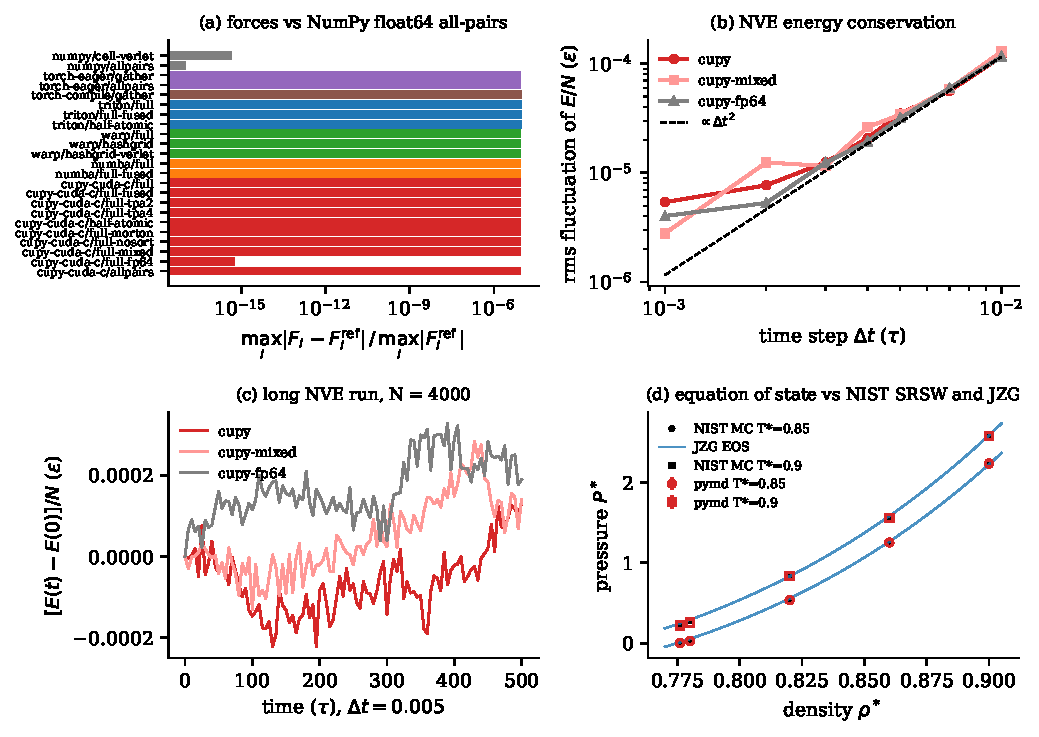
\includegraphics[width=\linewidth]{../figures/validation.pdf}
\caption{Validation. (a) Force error of every backend/variant versus the float64 oracle.
(b) Energy fluctuation versus time step. (c) Energy drift in a long NVE run for three
precisions. (d) Pressure versus NIST SRSW Monte Carlo data and the JZG equation of state.}
\label{fig:validation}
\end{figure}

\begin{figure}[htbp]
\centering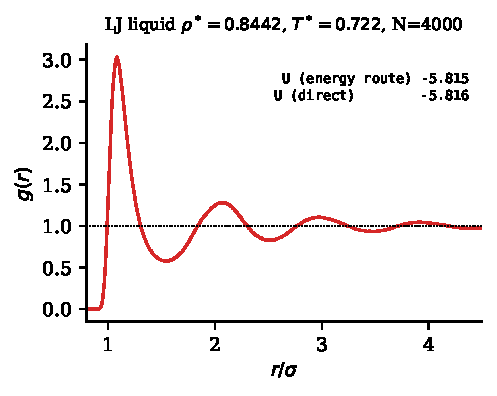
\includegraphics[width=0.6\linewidth]{../figures/rdf.pdf}
\caption{Radial distribution function of the LJ liquid at $\rho^*=0.8442$, $T^*=0.722$.}
\label{fig:rdf}
\end{figure}

\section{Performance}\label{sec:perf}
All numbers are medians of five timed repeats of at least 0.5\,s each after warm-up (JIT and
compilation excluded), with the GPU synchronized around the timed region.
\Cref{fig:perf} shows throughput versus system size; \cref{fig:roofline} the roofline and the
fraction of copy bandwidth at $N=\refN$.

\begin{figure}[htbp]
\centering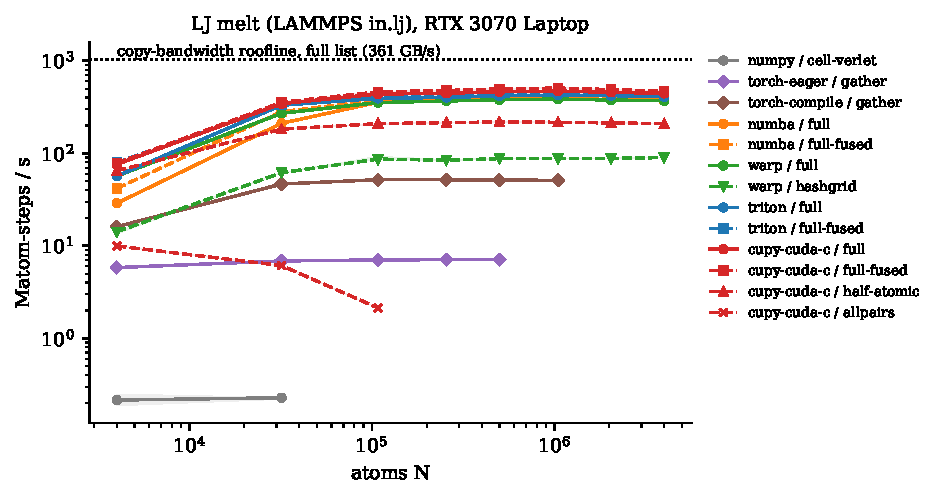
\includegraphics[width=\linewidth]{../figures/perf_vs_size.pdf}
\caption{Throughput on the \texttt{in.lj} melt versus atoms (bands: min--max of 5 repeats).
Dotted: the copy-bandwidth roofline of the minimal traffic model for a full list.}
\label{fig:perf}
\end{figure}

\begin{figure}[htbp]
\centering
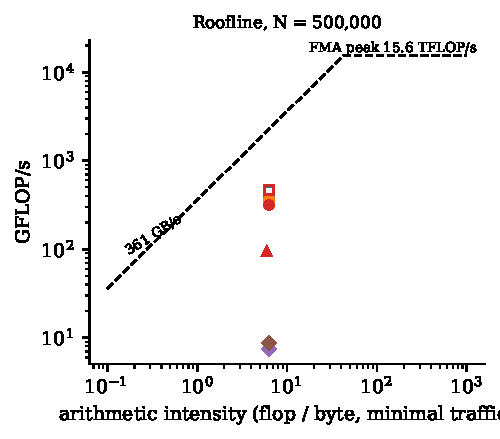
\includegraphics[width=0.49\linewidth]{../figures/roofline.pdf}\hfill
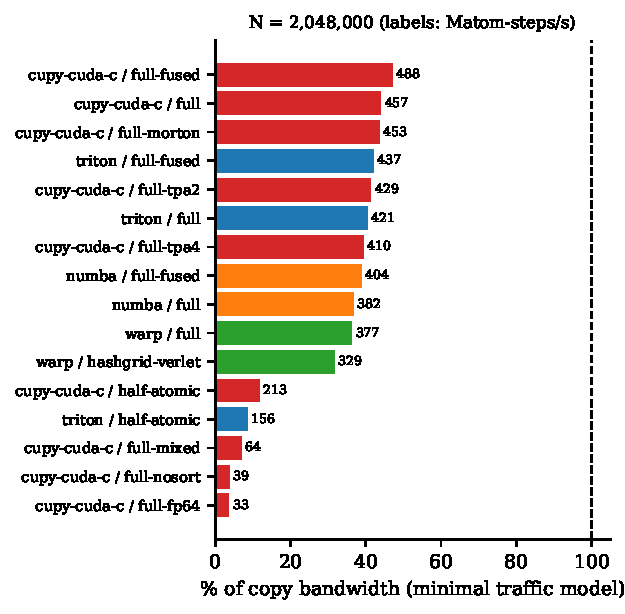
\includegraphics[width=0.49\linewidth]{../figures/roofline_bars.pdf}
\caption{Left: roofline (minimal traffic model) at $N=\refN$; filled markers unfused, open
markers fused kernels. Right: fraction of the \copyBW\,GB/s copy bandwidth.}
\label{fig:roofline}
\end{figure}

\paragraph{The ladder.} At $N=\refN$ the best variant per backend reaches (Matom-steps/s, \%
of copy bandwidth): Numba \refNumba{} (\refNumbaPct\%), Warp \refWarp{}
(\refWarpPct\%), Triton \refTriton{} (\refTritonPct\%) and CUDA C \refCupy{} (\refCupyPct\%).
The array rungs stop at smaller $N$ on the 8\,GB GPU: PyTorch eager reaches \refTorchEager{}
Matom-steps/s ($N=\refTorchEagerN$) and \texttt{torch.compile} \refTorchCompile{}
($N=\refTorchCompileN$, \refTorchCompilePct\%). The NumPy CPU baseline runs at \numpySmall{}
Matom-steps/s at $N=4000$. The array-programming
rungs are limited by the neighbor-list rebuild, which materializes candidate arrays; the
kernel languages share the same algorithm; we attribute their remaining differences to code
generation details such as vector versus scalar position loads and per-launch Python overhead
at small $N$ (we did not profile these in depth). The best overall is \bestBackend/\bestVariant{} with \bestRate{} Matom-steps/s at
$N=\bestN$ (\bestTauDay{} $\tau$/day, \bestNsDay{} ns/day for argon), \bestPctCopy\% of the
copy and \bestPctSpec\% of the specification bandwidth under our model.

\paragraph{Ablations} (\cref{fig:ablation}, CUDA C, $N=\ablN$, relative to \texttt{full}):
no spatial sorting \ablNoSortRatio$\times$, Morton order \ablMortonRatio$\times$ (row-major cell
order is already local at this cell size), half list with atomics \ablHalfRatio$\times$ (fewer
list bytes but three float atomics per pair), fused kernel \ablFusedRatio$\times$, two and four threads per atom
\ablTpaTwoRatio$\times$ and \ablTpaFourRatio$\times$, mixed
precision \ablMixedRatio$\times$ and fp64 \ablFpSixtyFourRatio$\times$ (the consumer GPU
executes fp64 at a small fraction of the fp32 rate).

\begin{figure}[htbp]
\centering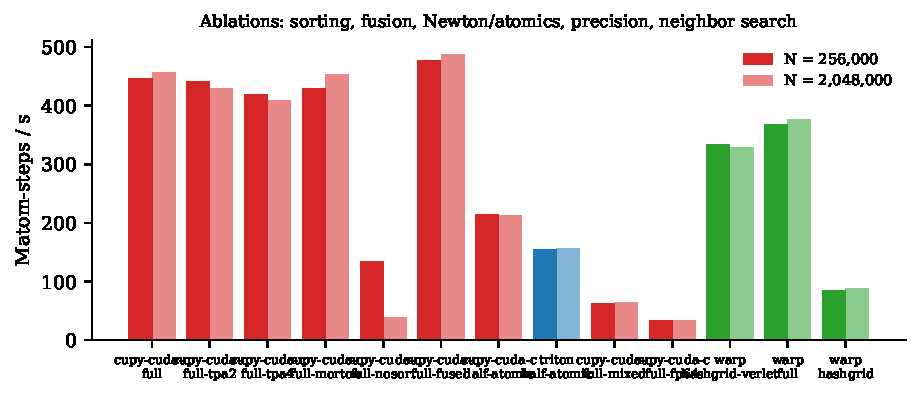
\includegraphics[width=\linewidth]{../figures/ablation.pdf}
\caption{Ablations at two sizes.}
\label{fig:ablation}
\end{figure}

\subsection{Same-GPU head-to-head with LAMMPS and HOOMD-blue}\label{sec:counterparts}
\ifnum\cpProvisional=1
\begin{center}
\fcolorbox{red}{red!8}{\parbox{0.92\linewidth}{\centering\bfseries\color{red!70!black}
PROVISIONAL --- the rates in this subsection come from the smoke run
\texttt{bench/counterparts.py --quick} ($N=\cpN$) on a GPU shared with other jobs.}}
\end{center}
\fi
Published rates of other codes are for other hardware, densities, cutoffs and precisions, so
we measure two established GPU MD codes on the same laptop GPU instead. LAMMPS
\lammpsVersion{} (\texttt{\lammpsTag})~\cite{thompson2022lammps} is built with CMake and
\texttt{nvcc}~\cpNvcc{} for \texttt{sm\_86} as a serial binary (MPI stubs, no OpenMP) in four
flavours: the GPU package~\cite{brown2011lammpsgpu} with \texttt{GPU\_PREC=mixed} and
\texttt{single}, and the KOKKOS package (Kokkos~5.2~\cite{trott2022kokkos}, CUDA back end) with
\texttt{KOKKOS\_PREC=double} and \texttt{single}. Each runs with its default package settings
(\texttt{-sf gpu -pk gpu 1}; \texttt{-k on g 1 -sf kk}, i.e.\ a full list with \texttt{newton
off}); for KOKKOS we also time a half list with \texttt{newton on}. HOOMD-blue
\hoomdVersion~\cite{anderson2020hoomd} is the conda-forge GPU build, which is compiled with a
64-bit \texttt{LongReal}, so its pair forces are evaluated in float64; for a like-for-like
comparison we also build the same release from source with \texttt{HOOMD\_LONGREAL\_SIZE=32}
(a one-line type fix in its GSD writer is needed to compile). All codes run the \texttt{in.lj}
problem of \cref{sec:method} with the same skin and the same unchecked rebuild every 20 steps
(HOOMD: \texttt{nlist.Cell(buffer=0.3, rebuild\_check\_delay=20, check\_dist=False)}).
LAMMPS creates its own lattice and velocities; HOOMD and \pymd{} start from \pymd's shuffled
lattice. LAMMPS rates are $N$ times steps over LAMMPS' own loop time of each of \cpRepeats{}
timed \texttt{run} commands after a warm-up run (setup excluded, as in its
\texttt{Performance} line); HOOMD rates come from the wall time of \texttt{Simulation.run}
after its autotuner has finished (up to 600\,s of tuning per size; it finished at every $N$ for
the single-precision build and at all but the two largest $N$ for the double-precision
build). The \pymd{} variants are timed in the same session.

\paragraph{Same system.} Before timing, every build integrates an identical initial state
(\cpVerN{} atoms, \pymd's lattice and velocities, read by LAMMPS through \texttt{read\_data} and
by HOOMD as a snapshot) for 100 steps. At step 0 the potential energy of every build agrees
with \pymd{} in float64 to $\le\num{\cpVerLammpsZeroEpot}$ (LAMMPS) and $\le\num{\cpVerHoomdZeroEpot}$
(HOOMD), and the pressure to $\le\num{\cpVerLammpsZeroPress}$ and $\le\num{\cpVerHoomdZeroPress}$; the
float32 builds set these maxima. After 100 steps all LAMMPS builds agree to
$\le\num{\cpVerLammpsHundredEpot}$ in energy and $\le\num{\cpVerLammpsHundredPress}$ in pressure, the same
level as \pymd's own float32 variant ($\num{\cpVerPymdSingleHundredEpot}$, $\num{\cpVerPymdSingleHundredPress}$).
HOOMD differs by up to $\num{\cpVerHoomdHundredEpot}$ and $\num{\cpVerHoomdHundredPress}$. This comes from
the benchmark's rebuild schedule, not from the force field: with rebuilds every 20 steps and no
displacement check, some pairs that cross the cutoff between rebuilds are missed, and which
ones depends on exactly when a code rebuilds. With the neighbor list kept complete (rebuild
checks every step), HOOMD agrees with \pymd{} to $\num{\cpVerHoomdEveryOneEpot}$ in energy.

\paragraph{Throughput.} At $N=\cpN$ (\cref{fig:counterparts}) the best \pymd{} variant
(\texttt{\cpPymdVariant}) runs at \cpPymd{} Matom-steps/s and the best Python kernel language
(\texttt{\cpPymdPythonVariant}) at \cpPymdPython. The fastest established code is
\cpCounterCode{} \texttt{\cpCounterVariant} (\cpCounterPrec{} precision) at \cpCounter{}
Matom-steps/s, so \pymd's best variant reaches \cpRatioCounter$\times$ and its best
Python-DSL variant \cpRatioPythonCounter$\times$ its throughput. HOOMD-blue runs at
\cpHoomdSingle{} Matom-steps/s in single precision and \cpHoomdDouble{} in the float64 conda
build. LAMMPS KOKKOS reaches \cpKokkosSingle{} (\texttt{\cpKokkosSingleVariant}) in single and
\cpKokkosDouble{} (\texttt{\cpKokkosDoubleVariant}) in double precision, the GPU package
\cpLmpGpu{} (\texttt{\cpLmpGpuVariant}), and LAMMPS on one CPU core \cpLmpCpu{} at
$N=\cpLmpCpuN$.

\paragraph{Why the codes differ.} (i) \emph{Precision.} Consumer Ampere GPUs execute float64
at a small fraction of the float32 rate, so every float64 build (HOOMD from conda-forge,
KOKKOS by default) is limited by double-precision arithmetic; \pymd's own float64 variant
(\ablFpSixtyFour{} Matom-steps/s at $N=\ablN$, \cref{fig:ablation}) is in the same range. The
float64 defaults are the right choice for data-centre GPUs; here single precision is
\cpHoomdPrecRatio$\times$ faster for HOOMD-blue and \cpKokkosPrecRatio$\times$ for KOKKOS.
(ii) \emph{KOKKOS in single precision.} \texttt{KOKKOS\_PREC=single} makes the pair arithmetic
float32, but the neighbor-list build still computes pair distances in float64 (the kernels in
\texttt{npair\_kokkos.cpp} cast positions to \texttt{double}), and on GPUs it bins atoms with a
bin edge of a full neighbor cutoff. In a development profile at $N=256{,}000$ (Nsight
Systems, shared GPU) this build, run every 20 steps by the benchmark, took most of KOKKOS' GPU
time, more than the force kernel. A half-cutoff bin size and \texttt{neigh/thread on} did not help in development runs, so
the benchmark keeps the defaults plus the half-list variant. (iii) \emph{GPU package.} Only the
pair force and the neighbor list run on the GPU (with binning on the host); time integration
(\texttt{fix nve/gpu}) runs on the CPU, and positions and forces cross PCIe every step. The package is designed for
several MPI ranks sharing one GPU to hide this, which a serial build cannot do. (iv)
\emph{HOOMD-blue in single precision} keeps all data on the GPU, uses full neighbor lists and
autotunes its launch parameters, as \pymd{} does, and is the closest counterpart. Its
remaining difference to \pymd{} comes from implementation details (list layout, number of
kernels per step, sorting policy) that we did not profile in depth. At small $N$, per-step
launch overheads weigh more for codes that launch several kernels per step.

\begin{figure}[htbp]
\centering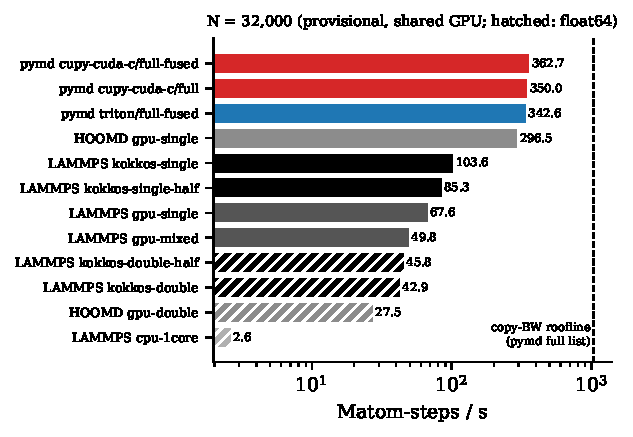
\includegraphics[width=\linewidth]{../figures/counterparts.pdf}
\caption{Same-GPU comparison on the \texttt{in.lj} melt: \pymd{} (backend colors) versus
LAMMPS \lammpsVersion{} (GPU and KOKKOS packages, one CPU core) and HOOMD-blue \hoomdVersion{}
(black and grey). Hatched bars and open markers: float64 arithmetic. Dashed: copy-bandwidth
roofline of \pymd's full-list traffic model (it does not apply to the other codes' layouts).}
\label{fig:counterparts}
\end{figure}

\paragraph{Published numbers.} For context only: Anderson et al.\ report 0.0778\,$\mu$s per
particle and step for an LJ liquid at $\rho^*=0.382$, $r_c=3\sigma$ (43.2 neighbors per
particle) on a GeForce 8800\,GTX in 2008~\cite{anderson2008hoomd}, and Anderson, Glaser and
Glotzer report $275\times10^6$ particle time steps per second for $N=64{,}000$ at the same
density, $k_BT=1.2$, on a single V100 GPU~\cite{anderson2020hoomd}. The archived LAMMPS
benchmark page lists 2.35\,s for 100 steps of the 1-million-atom \texttt{in.lj} problem on one
Tesla M2090 (2012)~\cite{lammps_bench_archive}, i.e.\ about 43 Matom-steps/s, and the LAMMPS
reference log of \texttt{in.lj} reports 3.752 Matom-step/s on one CPU core~\cite{lammps_inlj}.

\subsection{Head-to-head with the C++ predecessor \yamd}\label{sec:yamd}
\yamd's MPI-free library sources compile unchanged with \texttt{g++ -O3 -march=native}
(its meson build requires MPI, which is not installed, and an Eigen subproject that is
incomplete in the repository; we use the Eigen~3.4.0 tarball from its package cache, whose
hash matches the wrap file). Both codes then run identical open-boundary systems on the same
machine (\cref{fig:yamd}). Forces agree to \yamdForceDiff{} (LJ) and \yamdEamForceDiff{} (EAM)
absolute. For an FCC block of \yamdN{} atoms, single-threaded \yamd{} (neighbor list rebuilt
every step without skin, as \yamd{} does) runs at \yamdRate{} Matom-steps/s; the same
algorithm in NumPy runs at \yamdNumpySame{} (\yamdNumpySameRatio$\times$ slower than C++) and
on the GPU (CUDA C) at \yamdCupySame{} (\yamdCupySameRatio$\times$ faster). With \pymd's own
skin and rebuild schedule the GPU reaches \yamdCupyDefault{}. For a \yamdEamN-atom gold
cluster \yamd{} runs EAM at \yamdEamRate{} and the GPU at \yamdEamGpu{} Matom-steps/s. These
are apples-to-oranges comparisons (one CPU core versus a GPU; different neighbor-list
policies) included to document the lineage; the CPU is an \yamdCpu, otherwise idle during
the measurement.

\begin{figure}[htbp]
\centering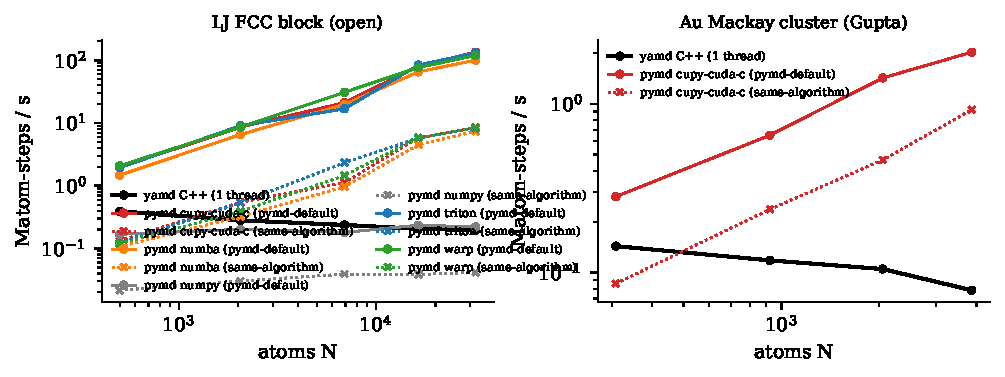
\includegraphics[width=\linewidth]{../figures/yamd_compare.pdf}
\caption{Same-machine comparison with the C++ code \yamd{} (single thread). ``same-algorithm'':
neighbor list rebuilt every step without skin, as in \yamd; ``pymd-default'': skin and
rebuild schedule of \pymd.}
\label{fig:yamd}
\end{figure}

\section{Discussion}
\paragraph{Where the time goes.} With sorted atoms the force kernel streams the neighbor index
list and hits cache for neighbor positions; the list bytes dominate the minimal model. The
remaining gap to the bandwidth ceiling is latency of dependent gathers (index, then position)
with one thread per atom; assigning two or four threads to each atom (the \texttt{full-tpa}
variants) raises memory-level parallelism but adds a shuffle reduction and partially idle lanes. Half lists halve the
index traffic but the atomic scatter costs more than it saves on this GPU.

\paragraph{Threats to validity.} (i) A single laptop GPU; laptop GPUs throttle under sustained
load, and clocks were not locked. (ii) Development timings were taken on a GPU shared with
other jobs; the published table comes from a serial run on an idle GPU. (iii) CUDA C is compiled by NVRTC through CuPy,
not \texttt{nvcc}; code generation is the same compiler back end but flags differ.
(iv) The traffic model excludes neighbor-position gathers and rebuilds, so percentages are
lower bounds on achieved bandwidth, and they are not comparable across codes that use
different list layouts. (v) Published numbers of other codes are for different densities,
cutoffs, precisions and hardware; this is why \cref{sec:counterparts} measures LAMMPS and
HOOMD-blue on our GPU. (vi) The \yamd{} comparison mixes CPU and GPU. (vii) We built and ran
LAMMPS and HOOMD-blue ourselves with their default settings plus the variants listed; experts
may tune them further (e.g.\ several MPI ranks per GPU for the LAMMPS GPU package, which our
serial build cannot use), and the source build of HOOMD-blue in single precision is not an
official binary.

\section{Conclusion}
Python kernel languages are not a compromise for short-range MD: on the LAMMPS LJ benchmark
Triton, Warp and Numba reach a large fraction of a hand-written CUDA C implementation of the
same algorithm, and the best variant uses \bestPctCopy\% of the copy bandwidth under a
conservative model, with validation against LAMMPS, NIST and an equation of state. The
array-programming rungs (NumPy, PyTorch) are easy to write but are an order of magnitude or
more behind, mostly because neighbor search does not map well onto dense array operations.

\section*{Code availability}
\pymd{} is MIT-licensed at \url{https://github.com/walidhemati/pymd}. \texttt{bench/run.py --full}
regenerates the benchmark JSON, \texttt{pymd validate} the validation JSON,
\texttt{figures/make\_figures.py} all figures and the numbers in this paper.

\renewcommand{\bibfont}{\small}
\setlength{\bibsep}{2pt plus 1pt}
\bibliographystyle{unsrtnat}
\bibliography{references}
\end{document}
